\chapter{Intrusion Detection Systems}
\minitoc
\emph{In \label{chap:IDS} this chapter we will define Intrusion Detection Systems, present an overview of the different types of Intrusion Detection Systems.}

\section{The problem}

Let us first provide an analogue, real world example of the security problem. Suppose that one has just bought a brand new luxury sedan. After parking it into the garage box, one might decide to install new security locks on the garage box's door, because the old ones do not use the up-to-date security mechanisms. After making a call to the locksmith who installs the new locks, you are the only one possessing the new keys.

After all that said and done, one decides to go on vacation. When returning home after a few weeks because of nostalgia, one decides to make a ride is his new car. However, when opening the door of the garage box, one does not see his brand new car as expected, but rather an empty garage box. What's worse is that one does not only see an empty box, but also some shards of glass on the floor. That led one to believe that someone broke into your garage box, stole your car and vandalized some of your possessions.

A few weeks before, one received a brochure of a company that installs burglar alarms. However, one threw it away. The installation and monitoring would have cost just 20 dollars a month. Neglecting to install the system is a secret one would have to leave with for the rest of one's life.

Could one have prevented the burglary from happening if one had installed the alarm?  Maybe not completely, but no doubt the damage would be less. \\ \\
This real life example is the same analogy of what might happen to one's computer network. What's more is that the thief may be at one's network for a long time without noticing him. Firewalls are doing (if properly configured) a good job guarding one's front door, but do not alert in case there is a back door or hole in one's infrastructure. So it is important to realize that a firewall is not an intrusion detection system.

\section{Intrusion Detection}

The \label{sec:ID} above example illustrates the need for intrusion detection systems. An IDS is the technology aimed at providing a precise detection measure on any intrusion attempt. We distinguish two different types of IDS: host based (HIDS) and network based NIDS).

A host intrusion detection system takes a snapshot of your existing system files and matches it to the previous snapshot. If the critical system files were modified or deleted, the alert is sent to the administrator to investigate. A HIDS protects therefore only one host. This is in contrast to a NIDS, which protects an entire network.

A NIDS is a sort of outdoor surveillance system that examines the data traffic passing troughout a network for any signs of intrusion. The IDS consists of two parts: the server and the sensor. The server is a station that manages the incoming alerts and updates signatures on the sensor. 

The sensor is a monitoring agent (station) that is put onto any monitored network and raises alarms to the server if any data traffic matches some pre-defined rules. Advantages of NIDS are the easy deployment (it doesn't affect any existing systems) and detection of network-based attacks such as DOS attacks, fragmented packets, etc\ldots. Disadvantages however include more false alarms compared to a HIDS.


\section{The different types of IDS}

\subsection{Difference in detection method}

There exist two main types of intrusion detection systems: signature-based (SBS) and anomaly-based (ABS). Signature-based intrusion detection systems use on pattern-matching techniques: they contain a database of signatures of known attacks and try to match these data against the analyzed data. When a match is found, an alarm is raised \citep{Roberto}. One can compare this to an anti-virus scanner.

On the other hand, anomaly-based intrusion detection systems first build a model of the network describing the normal network traffic and then reports any behaviour that significantly differs from the model as an attack \citep{Roberto, windowssecurity2}.

\subsubsection{Anomaly-Based Intrusion Detection Systems}

We will provide a brief description about ABSs. There exist different types of ABSs, but in general terms, they all consist of the following basic parts:
\begin{description}
\item[Training / learning phase] The normal behaviour of the system is characterized and a corresponding model is built. This can be done automatically or manually, depending on the type of ABS used.
\item[Detection phase] Once the model is built, it is compared with the observed traffic. If the difference found exceeds a pre-defined threshold value, an alarm will be triggered.
\item[Threshold value]
\end{description}

In comparision to signatured based intrusion detection systems, the main benefit of anomaly-based detection techniques is that they are able to detect previously unseen intrusion events. However, the rate of false positives in anomaly-based systems is usually higher than in signature-based ones \citep{CandS}.

As my paper focuses on the signature-based intrusion detection systems, we won't look further into the subject of anomaly-based IDSs.

\subsubsection{Signature-Based Intrusion Detection Systems}

Signature-based schemes look for defined patterns, or signatures, within the analyzed data. Therefore, a signature database with known attacks is created beforehand \citep{CandS}. When a match has been found, it is logged and an alert is raised to the network manager.

Signature-based schemes provide very good detection results for specified, well-known attacks. However, they are not capable of detecting new, unfamiliar intrusions, even if they are built as minimum variants of already known attacks \citep{CandS}.

\subsection{Classification based on protective system}

\subsubsection{HIDS}

As described in section \ref{sec:ID}, a host-based intrusion detection system or HIDS monitors activity on a single host  \citep{Host1}. Therefore, they are installed on a single system, which is in most cases a server. Whereas a HIDS resides on a single computer, a network-based intrusion detection system or NIDS is installed on, for example, routers \citep{windowssecurity2}, although they can obviously also be installed on a dedicated computer system.

Host-based intrusion detection systems can be divided into four types \citep{Report}:
\begin{description}
\item[File system monitoring] \hfill \\
File system monitoring is the process of ensuring the integrity of files and directories. HIDS implementations that use filesystem monitoring compare the current status of files on a regulary basis with previously gathered statusses about these files. This way, when an attacker gains access to those files and changes them, it will be detected. File system monitoring can check files for different characteristics inlucding, but not limited to: permissions, inode number, Owner/Group, size, etc\ldots.
\item[Logfile analysers] \hfill \\
Logfile analysers analyse logfiles for patterns indicating suspicious activity (= intrusions). By analyzing logfiles and determing if intrusion attempts were logged, an IDS can warn system administrators.
\item[Connection analysers] \hfill \\
A connection analyser monitors connection attempts to and from a host. They detect incoming network connections to the host they run on. Network-based intrusion detection systems (NIDS) as discussed in section \ref{subsub:NIDS} such as Snort use this approach \citep{Snort}.
\item[Kernel-based IDSs] \hfill \\
Kernel-based IDSs detect malicious activity on a kernel level. It is an adoption to or adoption of an existing kernel to have the kernel itself detect intrusions. Anomaly detection is a popular detection method used in Kernel-based IDSs. There exist various anomaly detection methods: anomaly detection based on a user's system usage, anomaly detection on the order of system calls in processes and anomaly detection on the arguments of system calls in processes.
\end{description}

\begin{figure}[h]
    \centering
    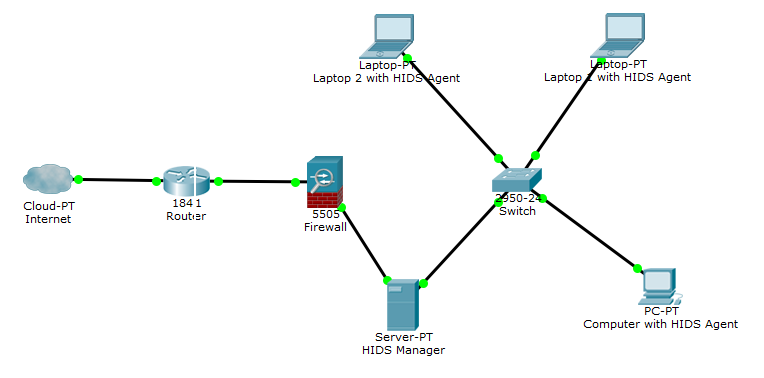
\includegraphics[width=0.85\textwidth]{HIDS.jpg}
    \caption{Example of a Host-based Intrusion Detection System}
    \label{fig:HIDS}
\end{figure}

Since Host-based IDSs are not designed to `see' network traffic, they are unable detect and report intrusions on a local network. That is when NIDS or Network-based intrusion detection systems come to help.

\subsubsection{NIDS}

A NIDS \label{subsub:NIDS} produces data about the local network. In particular, about local network usage. They collect information from the network itself, rather than from each seperate host \citep{Host2}. The NIDS analyze all network packets that reach the monitored network interface running in promiscuous mode \footnote{Promiscuous mode allows a network device to intercept and read each packet that arrives in its entity. I.e., it causes the network card to pass all traffic it receives to the CPU rather than passing only the frames that the controller is intended to receive. In a LAN, promiscuous mode is a mode of operation in which every data packet transmitted on the network can be received and read by the network adapter. Needless to say, promiscuous mode is used to monitor network traffic - and activity \citep{Prom}.}. Previous statement defines that a NIDS can not only be installed on a router, but also on a server that has a network interface card (NIC) operating in promiscuous mode.

Once a packet reaches the NIC, its header and content information is inspected \citep{Host2}. Signature-based IDSs come equipped with attack signatures, which are rules on what will constitute an attack. The sensors then compare these signatures to the traffic  that they capture. This method is known as packet sniffing \citep{Sniffing}.

\begin{figure}[h]
    \centering
    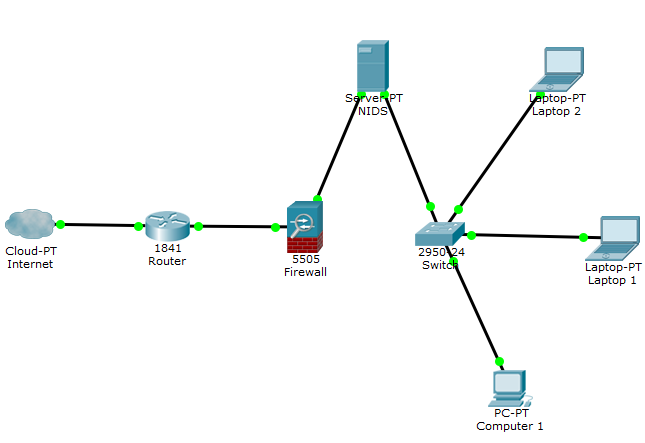
\includegraphics[width=0.85\textwidth]{NIDS.jpg}
    \caption{Example of a Network-based Intrusion Detection System}
    \label{fig:NIDS}
\end{figure}

